\documentclass[11pt]{article}

\usepackage[utf8]{inputenc}
\usepackage[T1]{fontenc}
\usepackage[francais]{babel}
\usepackage[top=1.8cm, bottom=1.8cm, left=1.8cm, right=1.8cm]{geometry}
\usepackage{hyperref}
\usepackage{graphicx}
\usepackage{epsfig}
\usepackage{array}
\hypersetup{
    colorlinks=true,
    breaklinks=true,
    urlcolor=red,
}
\parskip=5pt

\title{Organigramme}
\author{Pierre AYOUB, Claire BASKEVITCH, Tristan BESSAC, \\
Clément CAUMES, Damien DELAUNAY, Yassin DOUDOUH}
\date{Mercredi 14 Mars 2018}

\begin{document}
\hspace{1cm}
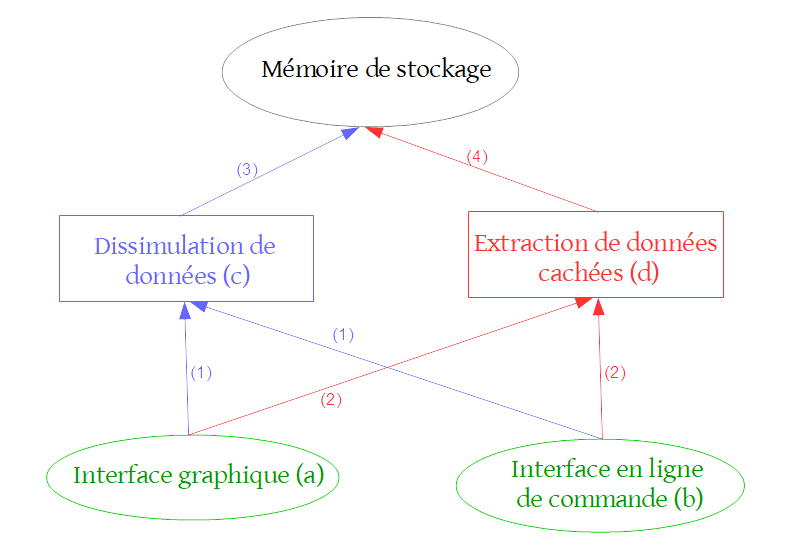
\includegraphics[scale=0.70]{organigramme.png}

\paragraph{Liste des modules et de leurs fonctionnalités}
\begin{description}
\item[a)] \textbf{Interface graphique} : interface permettant à l'utilisateur de choisir avec la souris parmi les deux fonctionnalités possibles de l'application. 
Il peut dissimuler des données dans un fichier (dont le type et le format sont pris en charge par l'application). Ou bien, il peut extraire les données cachées dans un fichier (s'il en dissimule). 

\item[b)] \textbf{Interface en ligne de commande} : interface ressemblante à celle graphique mais qui permet à l'utilisateur de manipuler l'application avec le terminal. 

\item[c)] \textbf{Dissimulation des données} : ce premier module implémente plusieurs fonctionnalités : 
\begin{itemize}
\item Compatibilité : le format du fichier "hôte" choisi par l'utilisateur est vérifié, pour savoir s'il est bien pris en charge par l'application. 
\item Proposition des algorithmes de stéganographie : en fonction du type et du format du fichier "hôte" ainsi que de la taille des données à cacher, un ou plusieurs algorithmes seront proposés. 
\item Insertion des données cachées dans l'hôte : écriture du fichier hôte dans lequel les données du fichier à cacher ont été insérées selon l'algorithme choisi par l'utilisateur. 
\end{itemize}

\item[d)] \textbf{Extraction des données} : ce deuxième module implémente aussi plusieurs fonctionnalités : 
\begin{itemize}
\item Compatibilité : le format du fichier "suspect" choisi par l'utilisateur doit être examiné afin de vérifier sa compatibilité avec l'application. 
\item Déterminisation : on recherche si le fichier suspect contient effectivement des données cachées. Cette déterminisation permet de savoir si un 
fichier a été utilisé par notre application dans le module \textit{Dissimulation des données (c)}.
Si le fichier suspect contient des données cachées, l'utilisateur choisira le chemin des données à extraire.
\item Extraction : écriture des données cachées présentes dans le fichier analysé (si le fichier suspect en contenait véritablement). 
\end{itemize}

\end{description}

\paragraph{Liste des informations qui circulent entre les modules}
\begin{description}
\item[1)] 
\begin{itemize}
\item fichier hôte 
\item fichier à cacher 
\item chemin et nom du fichier à créer, qui dissimulera les données à cacher et ayant l'apparence de l'hôte. 
\end{itemize}
\item[2)] 
\begin{itemize}
\item fichier suspect à analyser
\end{itemize}
\item[3)] 
\begin{itemize}
\item fichier hôte contenant les données cachées 
\end{itemize}
\item[4)]
\begin{itemize}
\item fichier résultant, représentant les données cachées 
\end{itemize}
\end{description}

\end{document}
